% !TeX spellcheck = en_GB

\section{GUI Tool: CYK Instances Generator }

\subsection{Overview GUI}
The tool consists out of four major elements as marked in Figure \ref{CYKInstancesGenerator}.
\begin{itemize}
	\item In area one elementary input values can be given to the programm.
	\item The status output of the programm is displayed at area two.
	\item Area 3 allows to automatically create suitable exercises to choose from.
	\item In area 4 the chosen exercise can be modified as wanted.
\end{itemize}
\begin{figure} [h]
	\centering
	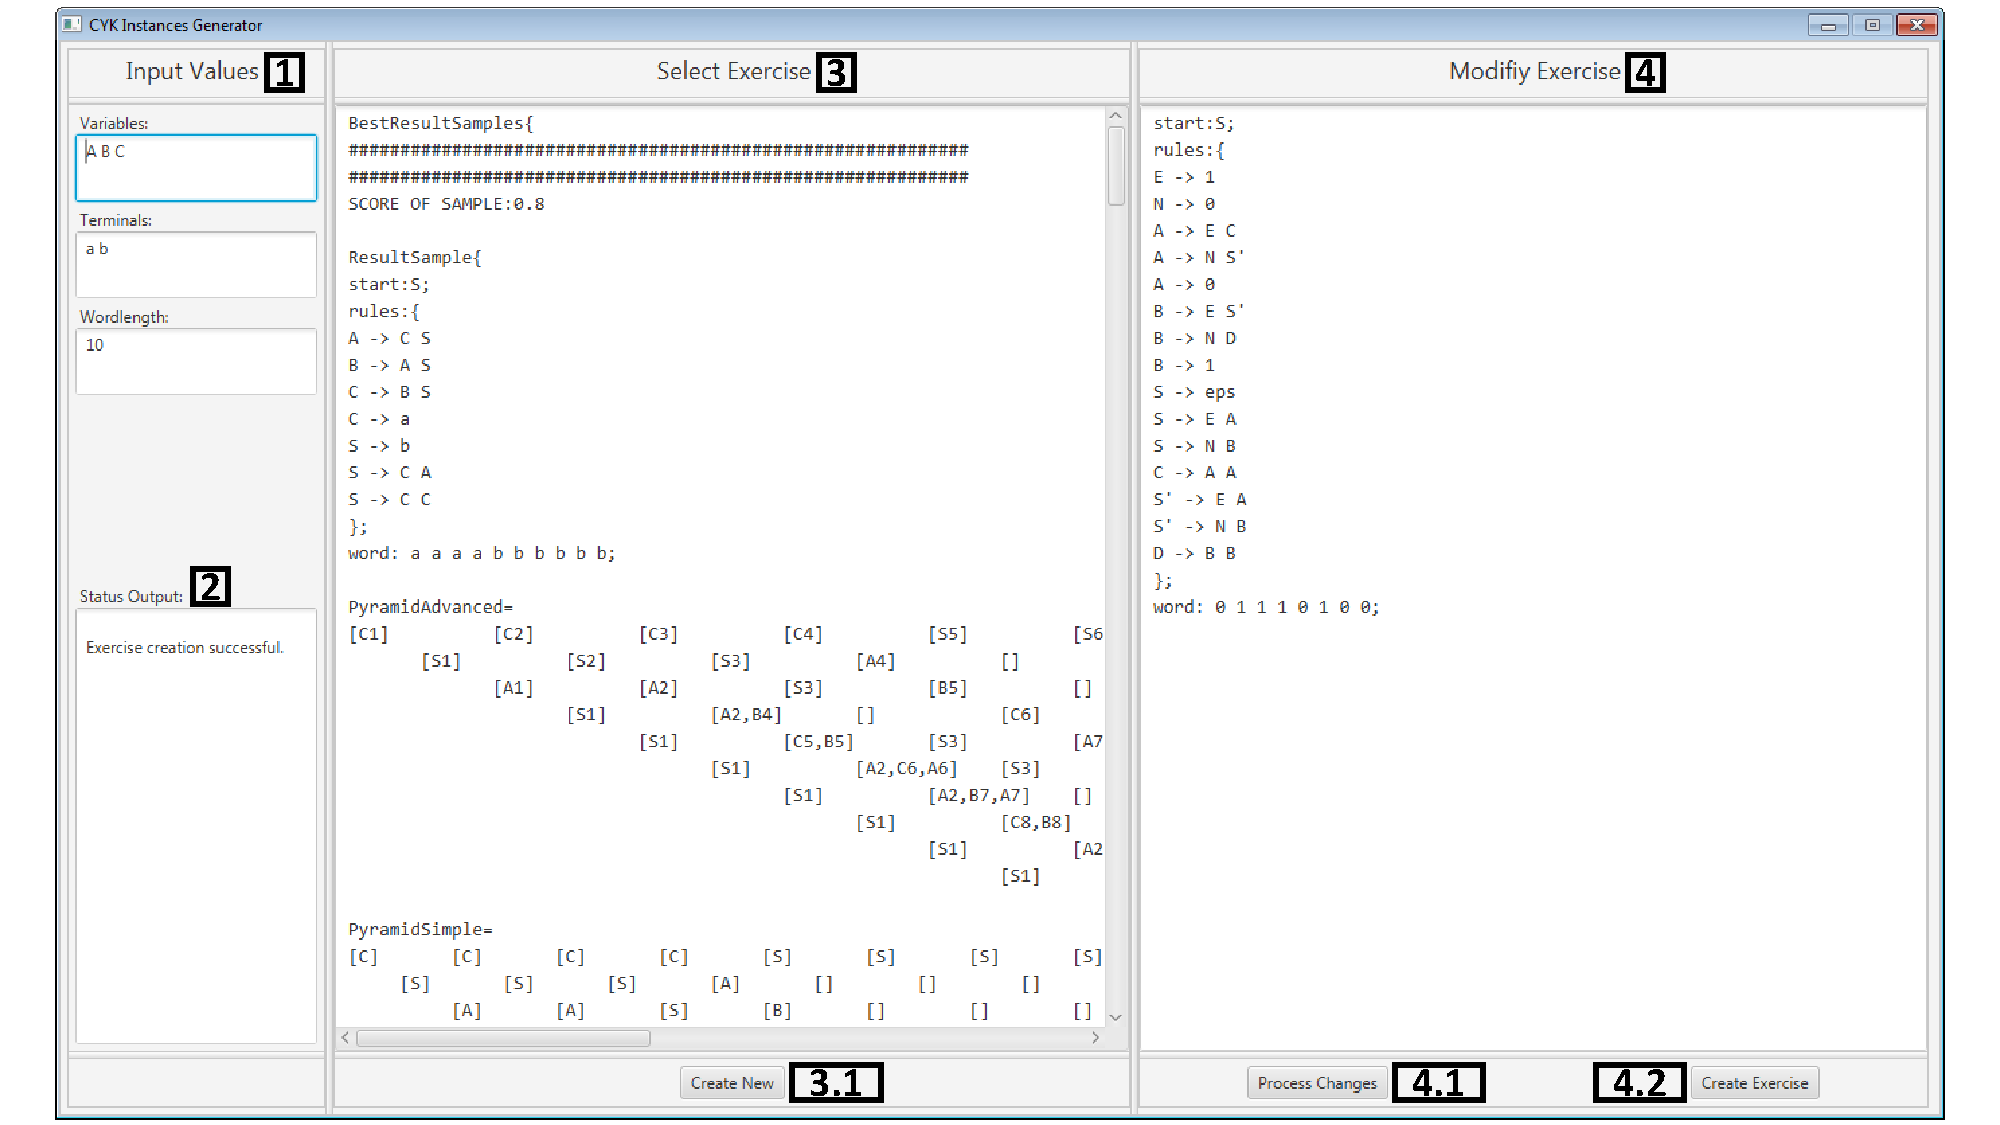
\includegraphics[width=\textwidth]{abb/CYKInstancesGenerator.pdf}
	\caption{CYK Instances Generator}
	\label{CYKInstancesGenerator}
\end{figure}
Clicking the button 3.1 allows the creation of new suitable exercises with the given input values from area 1. Pressing button 4.1 processes the latest input given in area 4 to create a preview analogously to area 3 of how the created exercise would look like and finally button 4.2 creates the desired $exercise$. The output for this $exercise$ is done through \LaTeX-code and a pdf-file.
\pagebreak
\subsection{Exam Exercises}
The 4-tuple $exercise = (grammar,\ word,\ parse\ table,\ derivation\ tree)$ that is the output of the tool looks as following:
\begin{figure} [h]
\begin{center} 
	\begin{tabular}{l}$E\rightarrow 1~~$\\ 
		$N\rightarrow 0~~$\\ 
		$A\rightarrow E C~|~N S'~|~0~~$\\ 
		$B\rightarrow E S'~|~N D~|~1~~$\\ 
		$S\rightarrow \epsilon~|~E A~|~N B~~$\\ 
		$C\rightarrow A A~~$\\ 
		$S'\rightarrow E A~|~N B~~$\\ 
		$D\rightarrow B B~~$\\ 
	\end{tabular} 
\end{center}
\begin{center}
	\resizebox{0.8\linewidth}{!}{
		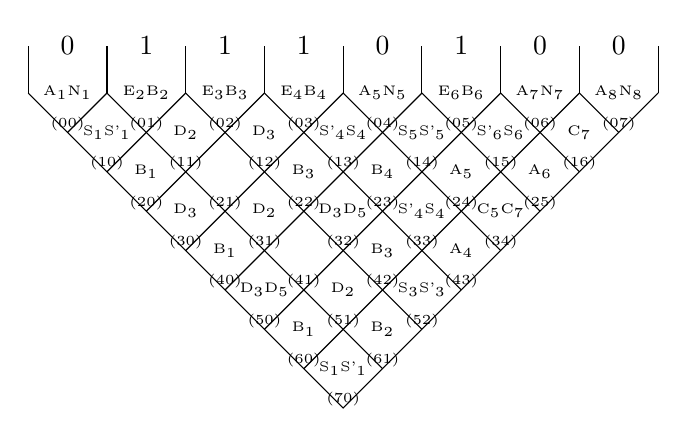
\begin{tikzpicture}[baseline]
		\newcommand{\myfontvars}[1]{
			\fontsize{4.9}{12}\selectfont{#1}
		}\newcommand{\myfontnumbering}[1]{
			\fontsize{2.5}{12}\selectfont{#1}
		}%Outer hull
		%Tip of the pyramid
		\coordinate (tip) at (4.0,-4.0);
		\foreach \i in {0,...,8} {
			\coordinate (\i) at (\i,0);
		}
		%Draw the left and right line of the pyramid pointing downwards
		\draw (0) -- (tip) -- (8);
		%Grid lines direction down-left to top-right
		\coordinate (dl1) at (0.5,-0.5);
		\coordinate (dl2) at (1.0,-1.0);
		\coordinate (dl3) at (1.5,-1.5);
		\coordinate (dl4) at (2.0,-2.0);
		\coordinate (dl5) at (2.5,-2.5);
		\coordinate (dl6) at (3.0,-3.0);
		\coordinate (dl7) at (3.5,-3.5);
		\draw (dl1) -- (1,0);
		\draw (dl2) -- (2,0);
		\draw (dl3) -- (3,0);
		\draw (dl4) -- (4,0);
		\draw (dl5) -- (5,0);
		\draw (dl6) -- (6,0);
		\draw (dl7) -- (7,0);
		%Grid lines direction down-right to top-left
		\coordinate (dr1) at (4.5,-3.5);
		\coordinate (dr2) at (5.0,-3.0);
		\coordinate (dr3) at (5.5,-2.5);
		\coordinate (dr4) at (6.0,-2.0);
		\coordinate (dr5) at (6.5,-1.5);
		\coordinate (dr6) at (7.0,-1.0);
		\coordinate (dr7) at (7.5,-0.5);
		\draw (dr1) -- (1,0);
		\draw (dr2) -- (2,0);
		\draw (dr3) -- (3,0);
		\draw (dr4) -- (4,0);
		\draw (dr5) -- (5,0);
		\draw (dr6) -- (6,0);
		\draw (dr7) -- (7,0);
		%Small lines at the top
		\coordinate (top0) at (0.0,0.0);
		\coordinate (top1) at (1.0,0.0);
		\coordinate (top2) at (2.0,0.0);
		\coordinate (top3) at (3.0,0.0);
		\coordinate (top4) at (4.0,0.0);
		\coordinate (top5) at (5.0,0.0);
		\coordinate (top6) at (6.0,0.0);
		\coordinate (top7) at (7.0,0.0);
		\coordinate (top8) at (8.0,0.0);
		\coordinate (topUpper0) at (0.0,0.6);
		\coordinate (topUpper1) at (1.0,0.6);
		\coordinate (topUpper2) at (2.0,0.6);
		\coordinate (topUpper3) at (3.0,0.6);
		\coordinate (topUpper4) at (4.0,0.6);
		\coordinate (topUpper5) at (5.0,0.6);
		\coordinate (topUpper6) at (6.0,0.6);
		\coordinate (topUpper7) at (7.0,0.6);
		\coordinate (topUpper8) at (8.0,0.6);
		\draw (top0) -- (topUpper0);
		\draw (top1) -- (topUpper1);
		\draw (top2) -- (topUpper2);
		\draw (top3) -- (topUpper3);
		\draw (top4) -- (topUpper4);
		\draw (top5) -- (topUpper5);
		\draw (top6) -- (topUpper6);
		\draw (top7) -- (topUpper7);
		\draw (top8) -- (topUpper8);
		%The string
		\coordinate (w0) at (0.5,0.6);
		\coordinate (w1) at (1.5,0.6);
		\coordinate (w2) at (2.5,0.6);
		\coordinate (w3) at (3.5,0.6);
		\coordinate (w4) at (4.5,0.6);
		\coordinate (w5) at (5.5,0.6);
		\coordinate (w6) at (6.5,0.6);
		\coordinate (w7) at (7.5,0.6);
		\node [] at (w0) {0};
		\node [] at (w1) {1};
		\node [] at (w2) {1};
		\node [] at (w3) {1};
		\node [] at (w4) {0};
		\node [] at (w5) {1};
		\node [] at (w6) {0};
		\node [] at (w7) {0};
		% Variables in the cells
		%cells00
		\coordinate (center00) at (0.5,0.0);
		\node [below=0.18cm] at (center00) {\myfontnumbering{$(00)$}};
		\node [] at (center00) {\myfontvars{A$_{1}$N$_{1}$}};
		%cells01
		\coordinate (center01) at (1.5,0.0);
		\node [below=0.18cm] at (center01) {\myfontnumbering{$(01)$}};
		\node [] at (center01) {\myfontvars{E$_{2}$B$_{2}$}};
		%cells02
		\coordinate (center02) at (2.5,0.0);
		\node [below=0.18cm] at (center02) {\myfontnumbering{$(02)$}};
		\node [] at (center02) {\myfontvars{E$_{3}$B$_{3}$}};
		%cells03
		\coordinate (center03) at (3.5,0.0);
		\node [below=0.18cm] at (center03) {\myfontnumbering{$(03)$}};
		\node [] at (center03) {\myfontvars{E$_{4}$B$_{4}$}};
		%cells04
		\coordinate (center04) at (4.5,0.0);
		\node [below=0.18cm] at (center04) {\myfontnumbering{$(04)$}};
		\node [] at (center04) {\myfontvars{A$_{5}$N$_{5}$}};
		%cells05
		\coordinate (center05) at (5.5,0.0);
		\node [below=0.18cm] at (center05) {\myfontnumbering{$(05)$}};
		\node [] at (center05) {\myfontvars{E$_{6}$B$_{6}$}};
		%cells06
		\coordinate (center06) at (6.5,0.0);
		\node [below=0.18cm] at (center06) {\myfontnumbering{$(06)$}};
		\node [] at (center06) {\myfontvars{A$_{7}$N$_{7}$}};
		%cells07
		\coordinate (center07) at (7.5,0.0);
		\node [below=0.18cm] at (center07) {\myfontnumbering{$(07)$}};
		\node [] at (center07) {\myfontvars{A$_{8}$N$_{8}$}};
		%cells10
		\coordinate (center10) at (1.0,-0.5);
		\node [below=0.18cm] at (center10) {\myfontnumbering{$(10)$}};
		\node [] at (center10) {\myfontvars{S$_{1}$S'$_{1}$}};
		%cells11
		\coordinate (center11) at (2.0,-0.5);
		\node [below=0.18cm] at (center11) {\myfontnumbering{$(11)$}};
		\node [] at (center11) {\myfontvars{D$_{2}$}};
		%cells12
		\coordinate (center12) at (3.0,-0.5);
		\node [below=0.18cm] at (center12) {\myfontnumbering{$(12)$}};
		\node [] at (center12) {\myfontvars{D$_{3}$}};
		%cells13
		\coordinate (center13) at (4.0,-0.5);
		\node [below=0.18cm] at (center13) {\myfontnumbering{$(13)$}};
		\node [] at (center13) {\myfontvars{S'$_{4}$S$_{4}$}};
		%cells14
		\coordinate (center14) at (5.0,-0.5);
		\node [below=0.18cm] at (center14) {\myfontnumbering{$(14)$}};
		\node [] at (center14) {\myfontvars{S$_{5}$S'$_{5}$}};
		%cells15
		\coordinate (center15) at (6.0,-0.5);
		\node [below=0.18cm] at (center15) {\myfontnumbering{$(15)$}};
		\node [] at (center15) {\myfontvars{S'$_{6}$S$_{6}$}};
		%cells16
		\coordinate (center16) at (7.0,-0.5);
		\node [below=0.18cm] at (center16) {\myfontnumbering{$(16)$}};
		\node [] at (center16) {\myfontvars{C$_{7}$}};
		%cells20
		\coordinate (center20) at (1.5,-1.0);
		\node [below=0.18cm] at (center20) {\myfontnumbering{$(20)$}};
		\node [] at (center20) {\myfontvars{B$_{1}$}};
		%cells21
		\coordinate (center21) at (2.5,-1.0);
		\node [below=0.18cm] at (center21) {\myfontnumbering{$(21)$}};
		%cells22
		\coordinate (center22) at (3.5,-1.0);
		\node [below=0.18cm] at (center22) {\myfontnumbering{$(22)$}};
		\node [] at (center22) {\myfontvars{B$_{3}$}};
		%cells23
		\coordinate (center23) at (4.5,-1.0);
		\node [below=0.18cm] at (center23) {\myfontnumbering{$(23)$}};
		\node [] at (center23) {\myfontvars{B$_{4}$}};
		%cells24
		\coordinate (center24) at (5.5,-1.0);
		\node [below=0.18cm] at (center24) {\myfontnumbering{$(24)$}};
		\node [] at (center24) {\myfontvars{A$_{5}$}};
		%cells25
		\coordinate (center25) at (6.5,-1.0);
		\node [below=0.18cm] at (center25) {\myfontnumbering{$(25)$}};
		\node [] at (center25) {\myfontvars{A$_{6}$}};
		%cells30
		\coordinate (center30) at (2.0,-1.5);
		\node [below=0.18cm] at (center30) {\myfontnumbering{$(30)$}};
		\node [] at (center30) {\myfontvars{D$_{3}$}};
		%cells31
		\coordinate (center31) at (3.0,-1.5);
		\node [below=0.18cm] at (center31) {\myfontnumbering{$(31)$}};
		\node [] at (center31) {\myfontvars{D$_{2}$}};
		%cells32
		\coordinate (center32) at (4.0,-1.5);
		\node [below=0.18cm] at (center32) {\myfontnumbering{$(32)$}};
		\node [] at (center32) {\myfontvars{D$_{3}$D$_{5}$}};
		%cells33
		\coordinate (center33) at (5.0,-1.5);
		\node [below=0.18cm] at (center33) {\myfontnumbering{$(33)$}};
		\node [] at (center33) {\myfontvars{S'$_{4}$S$_{4}$}};
		%cells34
		\coordinate (center34) at (6.0,-1.5);
		\node [below=0.18cm] at (center34) {\myfontnumbering{$(34)$}};
		\node [] at (center34) {\myfontvars{C$_{5}$C$_{7}$}};
		%cells40
		\coordinate (center40) at (2.5,-2.0);
		\node [below=0.18cm] at (center40) {\myfontnumbering{$(40)$}};
		\node [] at (center40) {\myfontvars{B$_{1}$}};
		%cells41
		\coordinate (center41) at (3.5,-2.0);
		\node [below=0.18cm] at (center41) {\myfontnumbering{$(41)$}};
		%cells42
		\coordinate (center42) at (4.5,-2.0);
		\node [below=0.18cm] at (center42) {\myfontnumbering{$(42)$}};
		\node [] at (center42) {\myfontvars{B$_{3}$}};
		%cells43
		\coordinate (center43) at (5.5,-2.0);
		\node [below=0.18cm] at (center43) {\myfontnumbering{$(43)$}};
		\node [] at (center43) {\myfontvars{A$_{4}$}};
		%cells50
		\coordinate (center50) at (3.0,-2.5);
		\node [below=0.18cm] at (center50) {\myfontnumbering{$(50)$}};
		\node [] at (center50) {\myfontvars{D$_{3}$D$_{5}$}};
		%cells51
		\coordinate (center51) at (4.0,-2.5);
		\node [below=0.18cm] at (center51) {\myfontnumbering{$(51)$}};
		\node [] at (center51) {\myfontvars{D$_{2}$}};
		%cells52
		\coordinate (center52) at (5.0,-2.5);
		\node [below=0.18cm] at (center52) {\myfontnumbering{$(52)$}};
		\node [] at (center52) {\myfontvars{S$_{3}$S'$_{3}$}};
		%cells60
		\coordinate (center60) at (3.5,-3.0);
		\node [below=0.18cm] at (center60) {\myfontnumbering{$(60)$}};
		\node [] at (center60) {\myfontvars{B$_{1}$}};
		%cells61
		\coordinate (center61) at (4.5,-3.0);
		\node [below=0.18cm] at (center61) {\myfontnumbering{$(61)$}};
		\node [] at (center61) {\myfontvars{B$_{2}$}};
		%cells70
		\coordinate (center70) at (4.0,-3.5);
		\node [below=0.18cm] at (center70) {\myfontnumbering{$(70)$}};
		\node [] at (center70) {\myfontvars{S$_{1}$S'$_{1}$}};
		\end{tikzpicture}
	}
\end{center}
\begin{center}
	\resizebox{0.45\linewidth}{!}{
		\begin{tikzpicture}[baseline]
		\tikzset{frontier/.style={distance from root=150pt}} %height of tree times 30pt
		\tikzset{edge from parent/.style= {
				draw,
				edge from parent path={(\tikzparentnode.south)	-- +(0,-8pt)-| (\tikzchildnode)}
			}
		}
		\Tree
		[.S1
		[.B1
		[.S1
		[.A1 0 ]
		[.B2 1 ]
		]
		[.E3 1 ]
		]
		[.A4
		[.S'4
		[.B4 1 ]
		[.N5 0 ]
		]
		[.A6
		[.S'6
		[.B6 1 ]
		[.A7 0 ]
		]
		[.N8 0 ]
		]
		]
		]
		\end{tikzpicture}
	}
\end{center}
\caption{Example output for a $exercise$.}
\label{exampleOutputExercise}
\end{figure}

\clearpage

\subsection{Scoring Model} \label{scoringMoetedel}
To be able to find suitable exercises that can be displayed in area 3 of the tool some kind of scoring is needed. ResultSamples are given a score according to Table \ref{scoring}. Parameter that will influence the score are:
\begin{itemize}
	\item RightCellCombinationsForcedCount
	\item maxSumOfVarsInPyramidCount 	
	\item maxNumberOfVarsPerCellCount
	\item maxSumOfProductionsCount
	\item homogeneity
	\item maxVarKsPerCell
\end{itemize}
\begin{table}[H]
	\centering
	\begin{tabular}{|l|c|c|c|c|c|l|}
		\hline
		\multicolumn{1}{|c|}{\multirow{2}{*}{Parameter}} & \multicolumn{6}{c|}{Points}                                                          \\ \cline{2-7} 
		\multicolumn{1}{|c|}{}		& 2          & 4           & 6           & 8           & 10          & -100            \\ \hline
		cellCombinationsForced      & {[}0,10{]} & {[}11,20{]} & {[}21,30{]} & {[}41,50{]} & {[}31,40{]} & \textgreater 50 \\ \hline
		sumVarsInPyramid            & {[}0,10{]} & {[}11,20{]} & {[}21,30{]} & {[}41,50{]} & {[}31,40{]} & \textgreater 50 \\ \hline
		maxVarsPerCell              & {[}5,5{]}  & {[}4,4{]}   & {[}1,1{]}   & {[}3,3{]}   & {[}2,2{]}   & \textgreater 5  \\ \hline
		sumProductions              & {[}1,2{]}  & {[}3,4{]}   & {[}5,6{]}   & {[}9,10{]}  & {[}7,8{]}   & \textgreater 10 \\ \hline
		homogeneity 				& {[} {]}  & {[} {]}   & {[} {]}   & {[} {]}  & {[} {]}   & \textgreater 10 \\ \hline
		maxVarKsPerCell 			& {[} {]}  & {[} {]}   & {[} {]}   & {[} {]}  & {[} {]}   & \textgreater 10 \\ \hline
	\end{tabular}
	\caption{Scoring of the different parameter values}
	\label{scoring}
\end{table}



\noindent Based on table \ref{scoring} each $exercise$ is scored.
The result will be normalized to the maximum possible points -> range 0.0 to 1.0. 

\pagebreak
\subsection{Parsing input with ANTLR}







\subsection{Other matters}

Technologies that have been used for programming are Github/Sourcetree, Maven, Intellij, ANTLR and JavaFX Scene Builder. [XXX] \\
Important used frameworks are: JUnit and Project Lombok. [XXX]\\
Altogether around 7100 lines of code have been written, of which 5400 are pure java code, 900 are comment lines and 800 are blank lines.\\

\subsubsection{Working with the program}
Short introduction on how to run the program and where to find the output exercise.
\pagebreak